\chapter{PARAMETERS}
\section{solver.ctqmc.in and solver.hfqmc.in}

In this section, we will introduce all of the parameters which can be used in the solver.ctqmc.in (for {\azalea}, {\gardenia}, {\narcissus}, {\begonia}, {\lavender}, {\pansy}, and {\manjushaka} components) and solver.hfqmc.in (for {\daisy} component) files. For more information, the uses can also refer to the comments in corresponding ctqmc\_control.f90 file.

\subsection{Jp}
{\color{red}DEFINITION:} Strength of pair-hopping term in the interaction term.

{\color{green}DATATYPE:} real(dp).

{\color{blue}DEFAULT:} 0.0\_dp.

{\color{brown}COMPONENT:} ALL, except for {\daisy}.

{\color{purple}BEHAVIOR:} Actually, this parameter is not used by the code internally. It will be outputted by the impurity solver as a reference.

{\color{olive}COMMENT:} NONE.

\subsection{Js}
{\color{red}DEFINITION:} Strength of spin-flip term in the interaction term.

{\color{green}DATATYPE:} real(dp).

{\color{blue}DEFAULT:} 0.0\_dp.

{\color{brown}COMPONENT:} ALL, except for {\daisy}.

{\color{purple}BEHAVIOR:} Actually, this parameter is not used by the code internally. It will be outputted by the impurity solver as a reference.

{\color{olive}COMMENT:} NONE.

\subsection{Jz}
{\color{red}DEFINITION:} Hund's exchange coupling constant.

{\color{green}DATATYPE:} real(dp).

{\color{blue}DEFAULT:} 0.0\_dp.

{\color{brown}COMPONENT:} ALL.

{\color{purple}BEHAVIOR:} In the {\azalea}, {\gardenia}, {\narcissus}, and {\daisy} codes, it is used to build the Coulomb interaction matrix. However, in the {\begonia}, {\lavender}, {\pansy}, and {\manjushaka} codes, this parameter is not used internally. It will be outputted by the impurity solver as a reference.

{\color{olive}COMMENT:} As for single-band model, $J_z = J_s = J_p = 0.0$. The condition $U_c = U_v - 2J_{z}$ should be always fulfilled.

\subsection{U}
{\color{red}DEFINITION:} Averaged Coulomb interaction.

{\color{green}DATATYPE:} real(dp).

{\color{blue}DEFAULT:} 4.0\_dp.

{\color{brown}COMPONENT:} ALL, except for {\daisy}.

{\color{purple}BEHAVIOR:} Actually, this parameter is not used by the code internally. It will be outputted by the impurity solver as a reference.

{\color{olive}COMMENT:} Usually, we let $U = U_c$.

\subsection{Uc}
{\color{red}DEFINITION:} Inter-orbital Coulomb interaction.

{\color{green}DATATYPE:} real(dp).

{\color{blue}DEFAULT:} 4.0\_dp.

{\color{brown}COMPONENT:} ALL.

{\color{purple}BEHAVIOR:} In the {\azalea}, {\gardenia}, {\narcissus}, and {\daisy} codes, it is used to build the Coulomb interaction matrix. However, in the {\begonia}, {\lavender}, {\pansy}, and {\manjushaka} codes, this parameter is not used internally. It will be outputted by the impurity solver as a reference.

{\color{olive}COMMENT:} The condition $U_c = U_v - 2J_{z}$ should be always fulfilled.

\subsection{Uv}
{\color{red}DEFINITION:} Intra-orbital Coulomb interaction.

{\color{green}DATATYPE:} real(dp).

{\color{blue}DEFAULT:} 4.0\_dp.

{\color{brown}COMPONENT:} ALL, except for {\daisy}.

{\color{purple}BEHAVIOR:} Actually, this parameter is not used by the code internally. It will be outputted by the impurity solver as a reference.

{\color{olive}COMMENT:} The condition $U_c = U_v - 2J_{z}$ should be always fulfilled.

\subsection{alpha}
{\color{red}DEFINITION:} Mixing parameter $\alpha$, used to mix the old and new self-energy function to produce a newer one.

{\color{green}DATATYPE:} real(dp).

{\color{blue}DEFAULT:} 0.7\_dp.

{\color{brown}COMPONENT:} ALL.

{\color{purple}BEHAVIOR:} $\Sigma_{\text{new}} = \alpha \Sigma_{\text{new}} + (1.0 - \alpha) \Sigma_{\text{old}}$

{\color{olive}COMMENT:} If you have trouble in obtaining convergence, you can decrease it to 0.5\_dp or even 0.2\_dp. If you are doing one-shot calculation (isscf = 1), this parameter is useless. 

\subsection{beta}
{\color{red}DEFINITION:} Inversion of temperature $\beta (= 1.0 / \text{T})$. Its unit is eV$^{-1}$.

{\color{green}DATATYPE:} real(dp).

{\color{blue}DEFAULT:} 8.0\_dp

{\color{brown}COMPONENT:} ALL.

{\color{purple}BEHAVIOR:} The impurity solver will use it to determine the system temperature.

{\color{olive}COMMENT:} The real temperature is 11604.505008098/$\beta$ Kelvin.

\subsection{chgrd}
{\color{red}DEFINITION:} Number of linear grid points in [-1,1].

{\color{green}DATATYPE:} integer.

{\color{blue}DEFAULT:} 20001.

{\color{brown}COMPONENT:} Only for {\gardenia}, {\narcissus}, {\lavender}, and {\manjushaka}.

{\color{purple}BEHAVIOR:} The second kind Chebyshev orthogonal polynomials are defined in a linear grid in [-1,1]. And the number of grid points are controlled by this parameter.

{\color{olive}COMMENT:} Only when isort = 3 or isort = 6 this parameter is useful. The 20001 is an optimal value for chgrd. It is not suggested to modified it. About the isort parameter, please refer to Sec.~\ref{subsec:isort}.

As for the applications of orthogonal polynomials in CT-QMC impurity solver, please refer to Phys. Rev. B 84. 075145 (2011) and Phys. Rev. B 85, 205106 (2012). 

\subsection{chmax}
{\color{red}DEFINITION:} The maximum allowable expansion order for the second kind Chebyshev orthogonal polynomials. It must be greater than 2.

{\color{green}DATATYPE:} integer.

{\color{blue}DEFAULT:} 32.

{\color{brown}COMPONENT:} Only for {\gardenia}, {\narcissus}, {\lavender}, and {\manjushaka}.

{\color{purple}BEHAVIOR:} The parameter is used as a cutoff to limit the maximum expansion order for the second kind Chebyshev orthogonal polynomials.

{\color{olive}COMMENT:} Only when isort = 3 or isort = 6 this parameter is useful. How to choose a suitable chmax parameters is a tricky job. If chmax is too small, the calculated results won't be accurate. If chmax is too large, the so-called Gibbs oscillation will occur dramatically. According to our experiences, 32 or 48 may be a reasonable choice. There is no upper limit. But the larger chmax, the heavier computational burden. About the isort parameter, please refer to Sec.~\ref{subsec:isort}.

As for the applications of orthogonal polynomials in CT-QMC impurity solver, please refer to Phys. Rev. B 84. 075145 (2011) and Phys. Rev. B 85, 205106 (2012).

\subsection{ifast}
{\color{red}DEFINITION:} Key control flag. It is used to select the suitable algorithm to calculate the operator trace. 

{\color{green}DATATYPE:} integer.

{\color{blue}DEFAULT:} 1.

{\color{brown}COMPONENT:} Only for {\manjushaka}.

{\color{purple}BEHAVIOR:} There are three possible values for ifast parameter so far:
\begin{itemize}
\item ifast = 1, the divide-and-conquer algorithm will be used. At this time, you have to adjust npart parameter carefully to obtain good computational efficiency.
\item ifast = 2, the classic time evolution algorithm will be used. WARNING: this algorithm is not implemented in the public version. We are sorry for that.
\item ifast = 3, the skip listing algorithm will be used. WARNING: this algorithm is not implemented in the public version. We are sorry for that.
\end{itemize}

All in all, now only ifast = 1 is valid. Even you set ifast = 2 or ifast = 3, {\manjushaka} code will still use the divide-and-conquer algorithm to calculate the operator trace.

{\color{olive}COMMENT:} In the {\manjushaka} code, the Lazy trace evaluation trick is always used.

As for the divide-and-conquer algorithm and the classic time evolution algorithm, please refer to Emanuel Gull's PhD thesis. As for the skip listing algorithm, please refer to Phys. Rev. B. 90 075149 (2014).

\subsection{isbin}
\begin{figure}
\centering
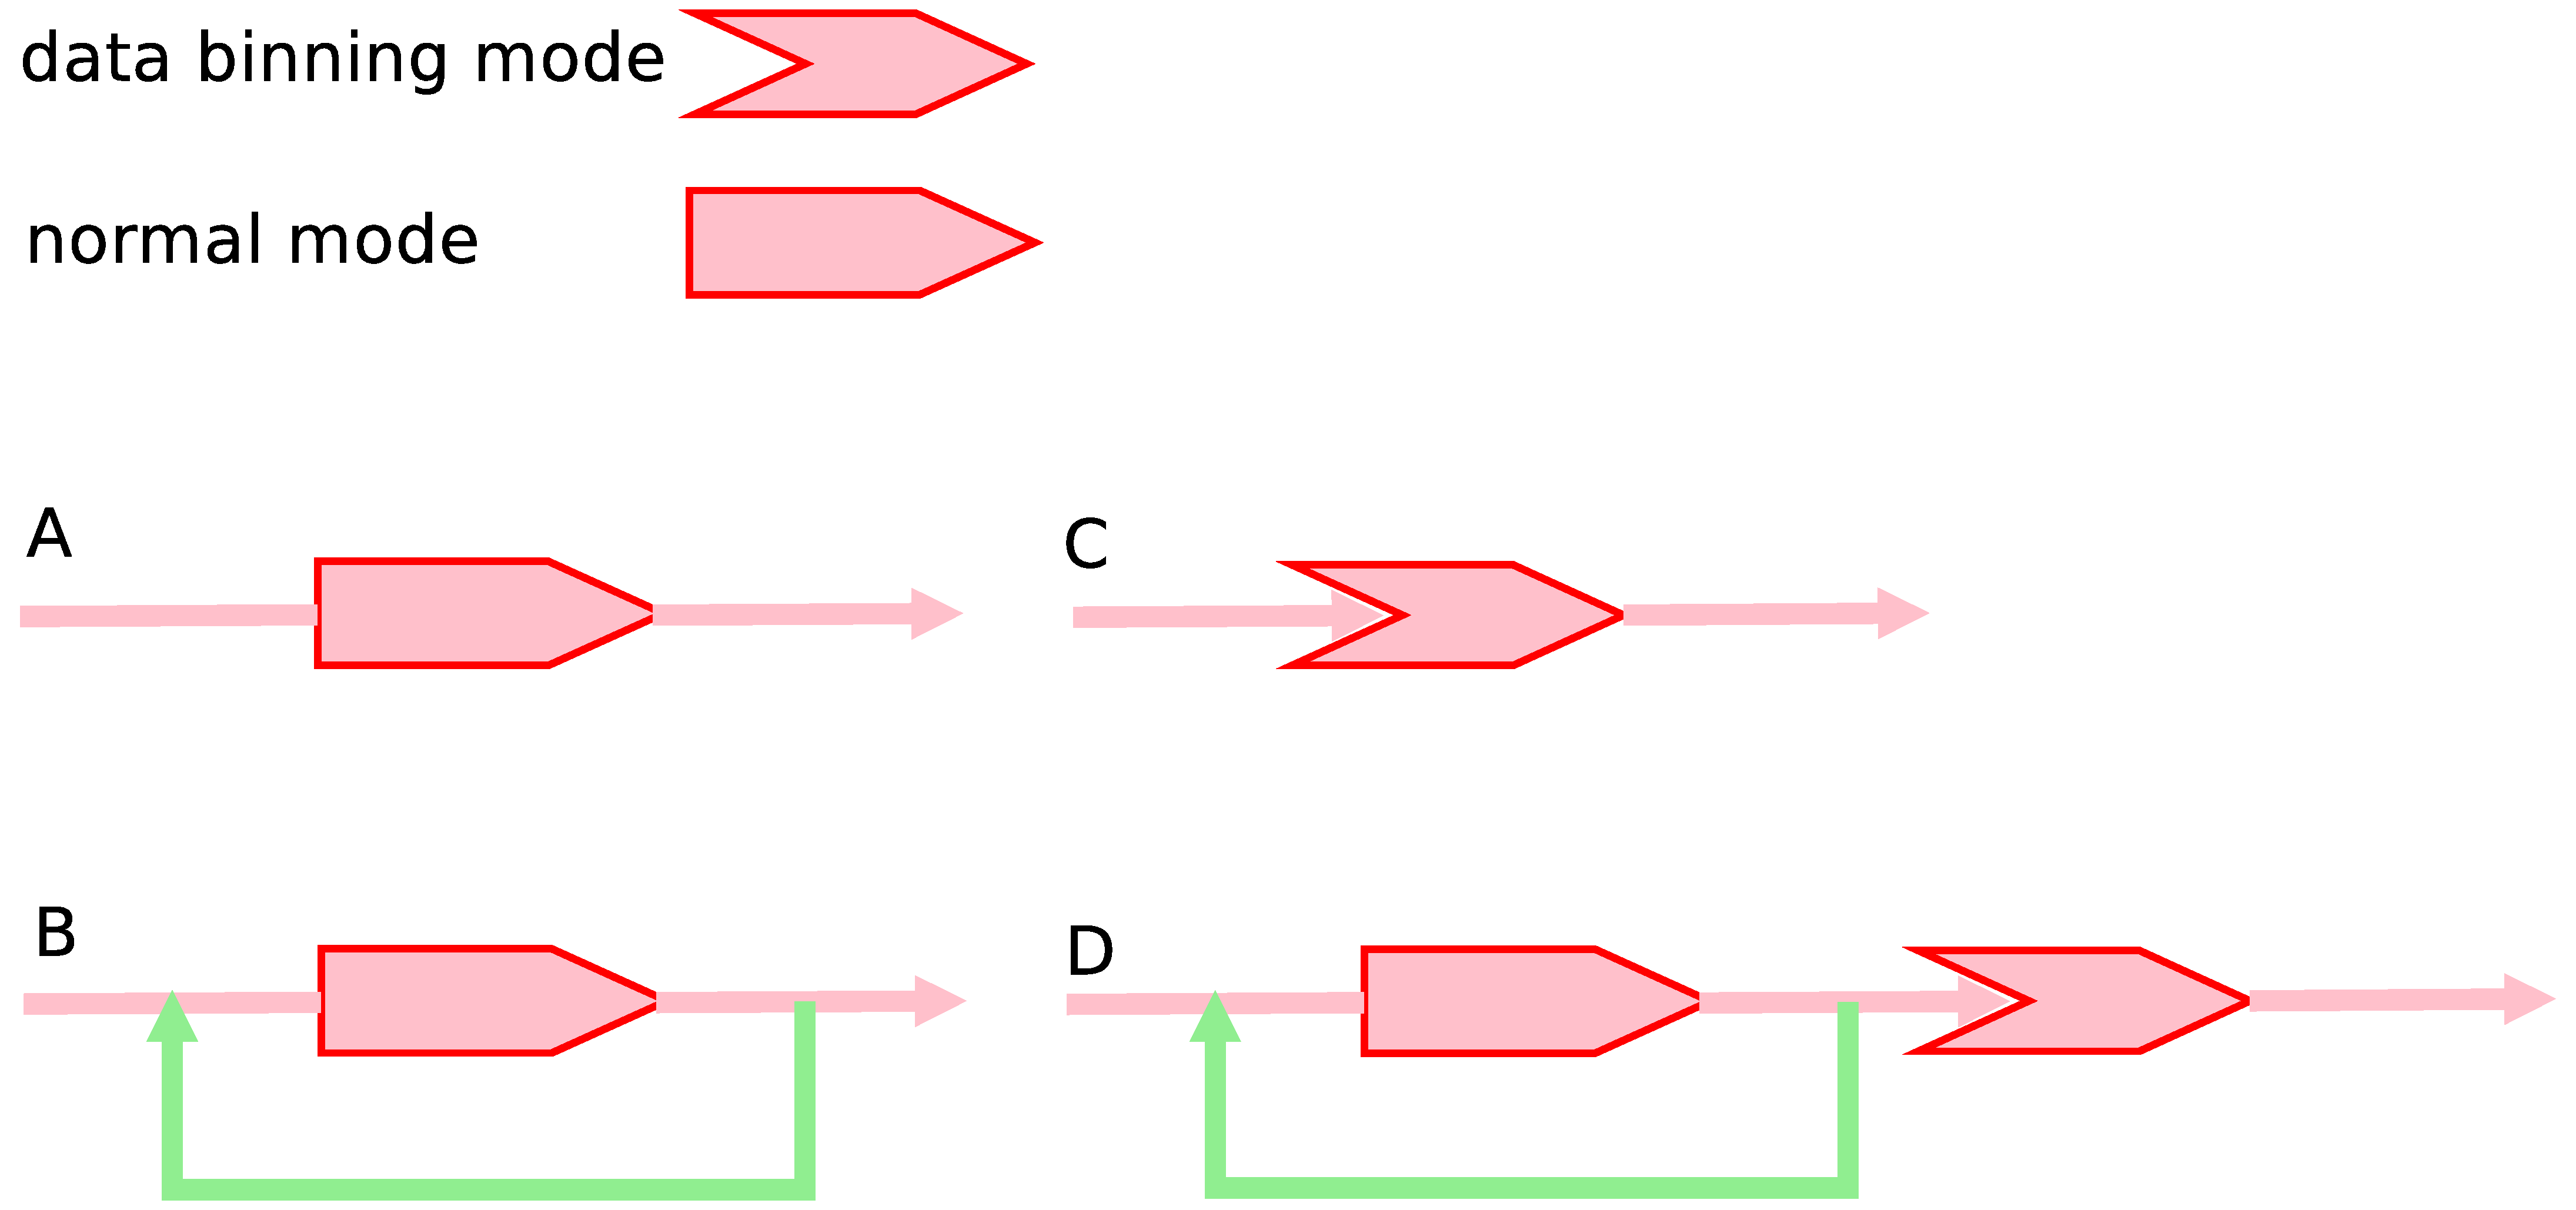
\includegraphics[scale=0.20]{figure/flow.eps}
\caption{The four running modes for quantum impurity solvers.\label{fig:flow}}
\end{figure}
{\color{red}DEFINITION:} Key control flag. It is used to determine whether we need to use the data binning mode.

{\color{green}DATATYPE:} integer.

{\color{blue}DEFAULT:} 2.

{\color{brown}COMPONENT:} ALL.

{\color{purple}BEHAVIOR:} There are three possible values for isbin parameter so far:
\begin{itemize}
\item isbin = 1, normal mode.
\item isbin = 2, data binning mode.
\end{itemize}
When the impurity solver is in the data binning mode, the current iteration number (iter, it is a internal variable) will be fixed to 999, nsweep and nwrite parameters will be increased by a factor of ten. The imaginary-time Green's function $G(\tau)$ will be outputted periodically to solver.green.bin.X files (where X denotes the index of data bins, from 1 to nsweep/nwrite), instead of solver.green.dat file. The post-processing tools will be used to deal with these files to do analytical continuation calculation.

{\color{olive}COMMENT:} From the combinations of isscf and isbin parameters, we can reach the following four running modes:
\begin{itemize}
\item A: isscf = 1, isbin = 1. The impurity solver is called only once. No DMFT self-consistent calculation. No data binning mode.
\item B: isscf = 2, isbin = 1. The impurity solves is called periodically in the DMFT self-consistent calculation. Once the convergence is reached, the calculation will be stopped. No data binning mode.   
\item C: isscf = 1, isbin = 2. The impurity solver is called only once in the data binning mode. No DMFT self-consistent calculation.
\item D: isscf = 2, isbin = 2. The impurity solves is called periodically in the DMFT self-consistent calculation. During the iterations, the impurity solver is in normal mode. After the convergence is reached, the impurity solver will be called once again. But at this time, the data binning mode is activated automatically.
\end{itemize}

Please see Fig.~\ref{fig:flow} for a intuitive view of the four running modes. If we want to perform LDA + DMFT calculations, mode A will be a good choice. Mode B is often used to solve model Hamiltonians iteratively and quickly to judge whether the results are reasonable. Once the results are reasonable and what we expect, and we want more accurate data, then we can use mode C. Mode D can be viewed as a combination of mode B and mode C, it is seldom used.

\subsection{isort\label{subsec:isort}}
{\color{red}DEFINITION:} Key control flag. It is used to determine whether we should use the orthogonal polynomials trick to improve the accuracy and suppress the numerical noises.

{\color{green}DATATYPE:} integer.

{\color{blue}DEFAULT:} 1.

{\color{brown}COMPONENT:} Only for {\gardenia}, {\narcissus}, {\lavender}, and {\manjushaka}.

{\color{purple}BEHAVIOR:} There are six possible values for isort parameter so far:
\begin{itemize}
\item isort = 1, the standard method is used to measure $G(\tau)$.
\item isort = 2, the Legendre orthogonal polynomials trick is used to measure $G(\tau)$.
\item isort = 3, the Chebyshev orthogonal polynomials trick is used to measure $G(\tau)$.
\item isort = 4, the standard method is used to measure $G(\tau)$ and $F(\tau)$
\item isort = 5, the Legendre orthogonal polynomials trick is used to measure $G(\tau)$ and $F(\tau)$.
\item isort = 6, the Chebyshev orthogonal polynomials trick is used to measure $G(\tau)$ and $F(\tau)$.
\end{itemize}
Here $G(\tau)$ is the imaginary-time Green's function and $F(\tau)$ auxiliary imaginary-time function which can be used to calculate $\Sigma(i\omega_n)$ analytically\footnote{Only when the Coulomb interaction matrix is density-density type, and {\gardenia} or {\narcissus} component is used.}.

{\color{olive}COMMENT:}

\subsection{isscf\label{subsec:isscf}}
{\color{red}DEFINITION:}

{\color{green}DATATYPE:} integer.

{\color{blue}DEFAULT:} 2.

{\color{brown}COMPONENT:} ALL.

{\color{purple}BEHAVIOR:}
\begin{itemize}
\item isscf = 1,
\item isscf = 2,
\end{itemize}

{\color{olive}COMMENT:}

\subsection{isscr\label{subsec:isscr}}
{\color{red}DEFINITION:}

{\color{green}DATATYPE:} integer.

{\color{blue}DEFAULT:} 1.

{\color{brown}COMPONENT:} Only for {\narcissus}.

{\color{purple}BEHAVIOR:}
\begin{itemize}
\item isscr = 1
\item isscr = 2
\item isscr = 3
\item isscr = 4
\item isscr = 99
\end{itemize}

{\color{olive}COMMENT:}

\subsection{isspn}
{\color{red}DEFINITION:}

{\color{green}DATATYPE:} integer.

{\color{blue}DEFAULT:} 1.

{\color{brown}COMPONENT:} ALL.

{\color{purple}BEHAVIOR:}
\begin{itemize}
\item isspn = 1,
\item isspn = 2,
\end{itemize}

{\color{olive}COMMENT:}

\subsection{issun}
{\color{red}DEFINITION:}

{\color{green}DATATYPE:} integer.

{\color{blue}DEFAULT:} 2.

{\color{brown}COMPONENT:} ALL.

{\color{purple}BEHAVIOR:}
\begin{itemize}
\item issun = 1,
\item issun = 2,
\end{itemize}

{\color{olive}COMMENT:}

\subsection{isvrt}
{\color{red}DEFINITION:}

{\color{green}DATATYPE:} integer.

{\color{blue}DEFAULT:}

{\color{brown}COMPONENT:} Only for {\gardenia}, {\narcissus}, {\lavender}, and {\manjushaka}.

{\color{purple}BEHAVIOR:}

{\color{olive}COMMENT:}

\subsection{itrun}
{\color{red}DEFINITION:} Key control flag. It is used to control which scheme should be used to truncate the Hilbert space.

{\color{green}DATATYPE:} integer.

{\color{blue}DEFAULT:} 1.

{\color{brown}COMPONENT:} Only for {\manjushaka}.

{\color{purple}BEHAVIOR:} There are two possible values for itrun parameter so far:
\begin{itemize}
\item itrun = 1, no truncation.
\item itrun = 2, those atomic states with low probability ($P_{\Gamma} < 1.0E-6$) will be truncated for next DMFT iteration.
\end{itemize}

{\color{olive}COMMENT:} This feature is experimental. Please check your calculated results carefully if you used the truncation approximation. To perform the truncation, the {\manjushaka} will read the solver.prob.dat file at first to get the probability data. So if this file is not available, the truncation will not be done.

To perform truncation over occupation number, you should use the {\jasmine} component to generate suitable atom.cix file.

\subsection{lc}
{\color{red}DEFINITION:} It is a model parameter for Hubbard-Holstein model or dynamical screening effect. The exact definition of lc depends on the value of isscr parameter.

{\color{green}DATATYPE:} real(dp).

{\color{blue}DEFAULT:} 1.0\_dp.

{\color{brown}COMPONENT:} Only for {\narcissus}.

{\color{purple}BEHAVIOR:}
\begin{itemize}
\item if isscr = 1, no meaning.
\item if isscr = 2, the $\lambda$ parameter in the Hubbard-Holstein model.
\item if isscr = 3, the $\lambda$ parameter in the plasmon-pole model for dynamical screening effect.
\item if isscr = 4, the $\alpha$ parameter in the ohmic model for dynamical screening effect.
\item if isscr = 99, shift for the chemical potential and Coulomb interaction (when we consider the dynamical screening effect in the LDA + DMFT calculations for realistic materials). You can obtain this value from the output of {\hibiscus}/toolbox/makescr.x.
\end{itemize}

{\color{olive}COMMENT:} Only when isscr $> 1$, it matters. As for the isscr parameter, please refer to Sec.~\ref{subsec:isscr}. About CT-QMC algorithm for Hubbard-Holstein model, please refer to Phys. Rev. Lett 99, 146404 (2007). About dynamical screening effect, plasmon-pole model, and ohmic mode, please refer to Phys. Rev. Lett. 104, 146401 (2010).

\subsection{legrd}
{\color{red}DEFINITION:} Number of linear grid points in [-1,1].

{\color{green}DATATYPE:} integer.

{\color{blue}DEFAULT:} 20001.

{\color{brown}COMPONENT:} Only for {\gardenia}, {\narcissus}, {\lavender}, and {\manjushaka}.

{\color{purple}BEHAVIOR:} The Legendre orthogonal polynomials are defined in a linear grid in [-1,1]. And the number of grid points are controlled by this parameter.

{\color{olive}COMMENT:} Only when isort = 2 or isort = 5 this parameter is useful. The 20001 is an optimal value for legrd. It is not suggested to modified it. About the isort parameter, please refer to Sec.~\ref{subsec:isort}.

As for the applications of orthogonal polynomials in CT-QMC impurity solver, please refer to Phys. Rev. B 84. 075145 (2011) and Phys. Rev. B 85, 205106 (2012). 

\subsection{lemax}
{\color{red}DEFINITION:} The maximum allowable expansion order for the Legendre orthogonal polynomials. It must be greater than 2.

{\color{green}DATATYPE:} integer.

{\color{blue}DEFAULT:} 32.

{\color{brown}COMPONENT:} Only for {\gardenia}, {\narcissus}, {\lavender}, and {\manjushaka}.

{\color{purple}BEHAVIOR:} The parameter is used as a cutoff to limit the maximum expansion order for the Legendre orthogonal polynomials.

{\color{olive}COMMENT:} Only when isort = 2 or isort = 5 this parameter is useful. How to choose a suitable lemax parameters is a tricky job. If lemax is too small, the calculated results won't be accurate. If lemax is too large, the so-called Gibbs oscillation will occur dramatically. According to our experiences, 32 or 48 may be a reasonable choice. It is worthy to emphasis that due to the limitation of implementation, lemax must be less than 50. About the isort parameter, please refer to Sec.~\ref{subsec:isort}.

As for the applications of orthogonal polynomials in CT-QMC impurity solver, please refer to Phys. Rev. B 84. 075145 (2011) and Phys. Rev. B 85, 205106 (2012).


\subsection{mfreq}
{\color{red}DEFINITION:} Number of matsubara frequency points.

{\color{green}DATATYPE:} integer.

{\color{blue}DEFAULT:} 8193 ($ = 2^{13} + 1)$.

{\color{brown}COMPONENT:} ALL.

{\color{purple}BEHAVIOR:} The $G(i\omega_n)$, $\mathcal{G}(i\omega_n)$, $\Sigma(i\omega_n)$, and $\Delta(i\omega_n)$ are all defined in this matsubara frequency grid.

{\color{olive}COMMENT:} It is an optimal value. Please do not modify it.

\subsection{mkink}
{\color{red}DEFINITION:} Maximum allowable diagrammatic perturbation order in the continuous-time quantum Monte Carlo algorithm.

{\color{green}DATATYPE:} integer.

{\color{blue}DEFAULT:} 1024.

{\color{brown}COMPONENT:} ALL, except for {\daisy}.

{\color{purple}BEHAVIOR:}

{\color{olive}COMMENT:} It is an optimal value. Please do not modify it.

\subsection{mstep}
{\color{red}DEFINITION:}

{\color{green}DATATYPE:} integer.

{\color{blue}DEFAULT:}

{\color{brown}COMPONENT:} Only for {\daisy}.

{\color{purple}BEHAVIOR:}

{\color{olive}COMMENT:}

\subsection{mune}
{\color{red}DEFINITION:} Chemical potential or Fermi level $\mu$.

{\color{green}DATATYPE:} real(dp)

{\color{blue}DEFAULT:} 2.0\_dp.

{\color{brown}COMPONENT:} ALL.

{\color{purple}BEHAVIOR:}

{\color{olive}COMMENT:} For single-band Hubbard mode, the half-filling condition is $\mu = U/2.0$.

\subsection{nband}
{\color{red}DEFINITION:} Number of bands ($N_{\text{band}}$).

{\color{green}DATATYPE:} integer.

{\color{blue}DEFAULT:} 1

{\color{brown}COMPONENT:} ALL.

{\color{purple}BEHAVIOR:}

{\color{olive}COMMENT:} In {\iqist}, when we say nband, we always do not consider the freedom of spin. So for $d-$electron system, it should be a five-band model (nband = 5), while for $f-$electron, it should be a seven-band model (nband = 7).

\subsection{nbfrq}
{\color{red}DEFINITION:} Number of bosonic frequencies.
 
{\color{green}DATATYPE:} integer.

{\color{blue}DEFAULT:} 4.

{\color{brown}COMPONENT:} Only for {\gardenia}, {\narcissus}, {\lavender}, and {\manjushaka}.

{\color{purple}BEHAVIOR:} The two-particle Green's function $\chi(i\omega,i\omega',i\nu)$ and vertex function $\mathcal{F}(i\omega,i\omega',i\nu)$ have three frequency indices where $\omega$ and $\omega'$ are fermionic frequencies, and $\nu$ bosonic frequency:
\begin{equation}
\nu_n = \frac{2n\pi}{\beta}
\end{equation}
\begin{equation}
\omega_n = \frac{(2n + 1)\pi}{\beta}
\end{equation}
The nbfrq parameter is used to define and generate $\nu_n$ bosonic mesh. The corresponding $\omega_n$ fermionic mesh is defined by nffrq parameter.

{\color{olive}COMMENT:} Usually nbfrq is small ( but nbfrq $> 0$ ), since the computational burden for two-particle quantities is extremely heavy.

\subsection{ncarlo}
{\color{red}DEFINITION:}

{\color{green}DATATYPE:} integer.

{\color{blue}DEFAULT:}

{\color{brown}COMPONENT:} ALL.

{\color{purple}BEHAVIOR:}

{\color{olive}COMMENT:}

\subsection{ncfgs}
{\color{red}DEFINITION:} Number of atomic configurations $N_{\text{cfgs}}$.

{\color{green}DATATYPE:} integer.

{\color{blue}DEFAULT:} 4.

{\color{brown}COMPONENT:} ALL.

{\color{purple}BEHAVIOR:} ncfgs = $2^{\text{norbs}}$.

{\color{olive}COMMENT:} Attention, the ncfgs should be consistent with nband, norbs, and nspin. The {\iqist} will not check the 
correctness of them.

\subsection{nclean}
{\color{red}DEFINITION:}

{\color{green}DATATYPE:} integer.

{\color{blue}DEFAULT:}

{\color{brown}COMPONENT:} ALL.

{\color{purple}BEHAVIOR:}

{\color{olive}COMMENT:}

\subsection{nffrq}
{\color{red}DEFINITION:} Number of fermionic frequencies.

{\color{green}DATATYPE:} integer.

{\color{blue}DEFAULT:} 32.

{\color{brown}COMPONENT:} ALL.

{\color{purple}BEHAVIOR:} The two-particle Green's function $\chi(i\omega,i\omega',i\nu)$ and vertex function $\mathcal{F}(i\omega,i\omega',i\nu)$ have three frequency indices where $\omega$ and $\omega'$ are fermionic frequencies, and $\nu$ bosonic frequency:
\begin{equation}
\nu_n = \frac{2n\pi}{\beta}
\end{equation}
\begin{equation}
\omega_n = \frac{(2n + 1)\pi}{\beta}
\end{equation}
The nffrq parameter is used to define and generate $\omega_n$ fermionic mesh. The corresponding $\nu_n$ bosonic mesh is defined by nbfrq parameter.

{\color{olive}COMMENT:} Usually nffrq is small ( but nffrq $> 0$ ), since the computational burden for two-particle quantities is extremely heavy.

\subsection{nflip}
{\color{red}DEFINITION:}

{\color{green}DATATYPE:} integer.

{\color{blue}DEFAULT:} 2000.

{\color{brown}COMPONENT:} ALL.

{\color{purple}BEHAVIOR:}

{\color{olive}COMMENT:}

\subsection{nfreq}
{\color{red}DEFINITION:}

{\color{green}DATATYPE:} integer.

{\color{blue}DEFAULT:} 128.

{\color{brown}COMPONENT:} ALL.

{\color{purple}BEHAVIOR:}

{\color{olive}COMMENT:}

\subsection{niter}
{\color{red}DEFINITION:} Number of DMFT self-consistent iterations.

{\color{green}DATATYPE:} integer.

{\color{blue}DEFAULT:} 20.

{\color{brown}COMPONENT:} ALL.

{\color{purple}BEHAVIOR:}

{\color{olive}COMMENT:}

\subsection{nmonte}
{\color{red}DEFINITION:}

{\color{green}DATATYPE:} integer.

{\color{blue}DEFAULT:}

{\color{brown}COMPONENT:} ALL.

{\color{purple}BEHAVIOR:}

{\color{olive}COMMENT:}

\subsection{norbs}
{\color{red}DEFINITION:} Number of orbitals ($N_{\text{orbs}}$).

{\color{green}DATATYPE:} integer.

{\color{blue}DEFAULT:} 2.

{\color{brown}COMPONENT:} ALL.

{\color{purple}BEHAVIOR:}

{\color{olive}COMMENT:}

\subsection{npart}
{\color{red}DEFINITION:}

{\color{green}DATATYPE:} integer.

{\color{blue}DEFAULT:} 4.

{\color{brown}COMPONENT:} ALL.

{\color{purple}BEHAVIOR:}

{\color{olive}COMMENT:}

\subsection{nsing}
{\color{red}DEFINITION:} Number of Ising auxiliary fields.

{\color{green}DATATYPE:} integer.

{\color{blue}DEFAULT:}

{\color{brown}COMPONENT:} Only for {\daisy}.

{\color{purple}BEHAVIOR:}

{\color{olive}COMMENT:}

\subsection{nspin}
{\color{red}DEFINITION:} Number of spin projections.

{\color{green}DATATYPE:} integer.

{\color{blue}DEFAULT:} 2.

{\color{brown}COMPONENT:} ALL.

{\color{purple}BEHAVIOR:}

{\color{olive}COMMENT:} DO NOT MODIFY IT. IT MUST BE 2 ALWAYS.

\subsection{nsweep}
{\color{red}DEFINITION:}

{\color{green}DATATYPE:} integer.

{\color{blue}DEFAULT:}

{\color{brown}COMPONENT:} ALL.

{\color{purple}BEHAVIOR:}

{\color{olive}COMMENT:}

\subsection{ntherm}
{\color{red}DEFINITION:} Number of thermalization (warmup) steps.

{\color{green}DATATYPE:} integer.

{\color{blue}DEFAULT:}

{\color{brown}COMPONENT:} ALL.

{\color{purple}BEHAVIOR:}

{\color{olive}COMMENT:}

\subsection{ntime}
{\color{red}DEFINITION:} Number of time slices.

{\color{green}DATATYPE:} integer.

{\color{blue}DEFAULT:}

{\color{brown}COMPONENT:} ALL.

{\color{purple}BEHAVIOR:}

{\color{olive}COMMENT:}

\subsection{nwrite}
{\color{red}DEFINITION:}

{\color{green}DATATYPE:} integer.

{\color{blue}DEFAULT:}

{\color{brown}COMPONENT:}

{\color{purple}BEHAVIOR:}

{\color{olive}COMMENT:}

\subsection{nzero}
{\color{red}DEFINITION:}

{\color{green}DATATYPE:} integer.

{\color{blue}DEFAULT:}

{\color{brown}COMPONENT:} Only for {\begonia} and {\lavender}.

{\color{purple}BEHAVIOR:}

{\color{olive}COMMENT:}

\subsection{part}
{\color{red}DEFINITION:} Hopping paramter $t$ in the Hubbard model

{\color{green}DATATYPE:} real(dp).

{\color{blue}DEFAULT:} 0.5\_dp

{\color{brown}COMPONENT:} ALL.

{\color{purple}BEHAVIOR:} This parameter is only used to initialize the initial hybridization function $\Delta(i\omega)$ and calculate new hybridization function through the self-consistent condition ($\Delta = t^2 G$, for bethe lattice).

{\color{olive}COMMENT:} This parameter has influences on the results only when isscf = 2. About the isscf parameter, please refer to Sec.~\ref{subsec:isscf}.

\subsection{wc}
{\color{red}DEFINITION:}

{\color{green}DATATYPE:} real(dp)

{\color{blue}DEFAULT:} 1.0\_dp

{\color{brown}COMPONENT:} Only for {\narcissus}.

{\color{purple}BEHAVIOR:}

{\color{olive}COMMENT:}

\section{entropy.in and sac.in}
\subsection{ainit}
{\color{red}DEFINITION:}

{\color{green}DATATYPE:}

{\color{blue}DEFAULT:}

{\color{brown}COMPONENT:}

{\color{purple}BEHAVIOR:}

{\color{olive}COMMENT:}

\subsection{beta}
{\color{red}DEFINITION:}

{\color{green}DATATYPE:}

{\color{blue}DEFAULT:}

{\color{brown}COMPONENT:}

{\color{purple}BEHAVIOR:}

{\color{olive}COMMENT:}

\subsection{devia}
{\color{red}DEFINITION:}

{\color{green}DATATYPE:}

{\color{blue}DEFAULT:}

{\color{brown}COMPONENT:}

{\color{purple}BEHAVIOR:}

{\color{olive}COMMENT:}

\subsection{eta1}
{\color{red}DEFINITION:}

{\color{green}DATATYPE:}

{\color{blue}DEFAULT:}

{\color{brown}COMPONENT:}

{\color{purple}BEHAVIOR:}

{\color{olive}COMMENT:}

\subsection{eta2}
{\color{red}DEFINITION:}

{\color{green}DATATYPE:}

{\color{blue}DEFAULT:}

{\color{brown}COMPONENT:}

{\color{purple}BEHAVIOR:}

{\color{olive}COMMENT:}

\subsection{legrd}
{\color{red}DEFINITION:}

{\color{green}DATATYPE:}

{\color{blue}DEFAULT:}

{\color{brown}COMPONENT:}

{\color{purple}BEHAVIOR:}

{\color{olive}COMMENT:}

\subsection{lemax}
{\color{red}DEFINITION:}

{\color{green}DATATYPE:}

{\color{blue}DEFAULT:}

{\color{brown}COMPONENT:}

{\color{purple}BEHAVIOR:}

{\color{olive}COMMENT:}

\subsection{ltype}
{\color{red}DEFINITION:}

{\color{green}DATATYPE:}

{\color{blue}DEFAULT:}

{\color{brown}COMPONENT:}

{\color{purple}BEHAVIOR:}

{\color{olive}COMMENT:}

\subsection{nalph}
{\color{red}DEFINITION:}

{\color{green}DATATYPE:}

{\color{blue}DEFAULT:}

{\color{brown}COMPONENT:}

{\color{purple}BEHAVIOR:}

{\color{olive}COMMENT:}

\subsection{nband}
{\color{red}DEFINITION:}

{\color{green}DATATYPE:}

{\color{blue}DEFAULT:}

{\color{brown}COMPONENT:}

{\color{purple}BEHAVIOR:}

{\color{olive}COMMENT:}

\subsection{ndump}
{\color{red}DEFINITION:}

{\color{green}DATATYPE:}

{\color{blue}DEFAULT:}

{\color{brown}COMPONENT:}

{\color{purple}BEHAVIOR:}

{\color{olive}COMMENT:}

\subsection{ngamm}
{\color{red}DEFINITION:}

{\color{green}DATATYPE:}

{\color{blue}DEFAULT:}

{\color{brown}COMPONENT:}

{\color{purple}BEHAVIOR:}

{\color{olive}COMMENT:}

\subsection{ngrid}
{\color{red}DEFINITION:}

{\color{green}DATATYPE:}

{\color{blue}DEFAULT:}

{\color{brown}COMPONENT:}

{\color{purple}BEHAVIOR:}

{\color{olive}COMMENT:}

\subsection{niter}
{\color{red}DEFINITION:}

{\color{green}DATATYPE:}

{\color{blue}DEFAULT:}

{\color{brown}COMPONENT:}

{\color{purple}BEHAVIOR:}

{\color{olive}COMMENT:}

\subsection{norbs}
{\color{red}DEFINITION:}

{\color{green}DATATYPE:}

{\color{blue}DEFAULT:}

{\color{brown}COMPONENT:}

{\color{purple}BEHAVIOR:}

{\color{olive}COMMENT:}

\subsection{nstep}
{\color{red}DEFINITION:}

{\color{green}DATATYPE:}

{\color{blue}DEFAULT:}

{\color{brown}COMPONENT:}

{\color{purple}BEHAVIOR:}

{\color{olive}COMMENT:}

\subsection{ntime}
{\color{red}DEFINITION:}

{\color{green}DATATYPE:}

{\color{blue}DEFAULT:}

{\color{brown}COMPONENT:}

{\color{purple}BEHAVIOR:}

{\color{olive}COMMENT:}

\subsection{ntune}
{\color{red}DEFINITION:}

{\color{green}DATATYPE:}

{\color{blue}DEFAULT:}

{\color{brown}COMPONENT:}

{\color{purple}BEHAVIOR:}

{\color{olive}COMMENT:}

\subsection{ntype}
{\color{red}DEFINITION:}

{\color{green}DATATYPE:}

{\color{blue}DEFAULT:}

{\color{brown}COMPONENT:}

{\color{purple}BEHAVIOR:}

{\color{olive}COMMENT:}

\subsection{nwarm}
{\color{red}DEFINITION:}

{\color{green}DATATYPE:}

{\color{blue}DEFAULT:}

{\color{brown}COMPONENT:}

{\color{purple}BEHAVIOR:}

{\color{olive}COMMENT:}

\subsection{nwmax}
{\color{red}DEFINITION:}

{\color{green}DATATYPE:}

{\color{blue}DEFAULT:}

{\color{brown}COMPONENT:}

{\color{purple}BEHAVIOR:}

{\color{olive}COMMENT:}

\subsection{ratio}
{\color{red}DEFINITION:}

{\color{green}DATATYPE:}

{\color{blue}DEFAULT:}

{\color{brown}COMPONENT:}

{\color{purple}BEHAVIOR:}

{\color{olive}COMMENT:}

\subsection{sigma}
{\color{red}DEFINITION:}

{\color{green}DATATYPE:}

{\color{blue}DEFAULT:}

{\color{brown}COMPONENT:}

{\color{purple}BEHAVIOR:}

{\color{olive}COMMENT:}

\subsection{wstep}
{\color{red}DEFINITION:}

{\color{green}DATATYPE:}

{\color{blue}DEFAULT:}

{\color{brown}COMPONENT:}

{\color{purple}BEHAVIOR:}

{\color{olive}COMMENT:}

\section{atom.config.in}
\subsection{Jh}
{\color{red}DEFINITION:}

{\color{green}DATATYPE:}

{\color{blue}DEFAULT:}

{\color{brown}COMPONENT:}

{\color{purple}BEHAVIOR:}

{\color{olive}COMMENT:}

\subsection{Jp}
{\color{red}DEFINITION:}

{\color{green}DATATYPE:}

{\color{blue}DEFAULT:}

{\color{brown}COMPONENT:}

{\color{purple}BEHAVIOR:}

{\color{olive}COMMENT:}

\subsection{Js}
{\color{red}DEFINITION:}

{\color{green}DATATYPE:}

{\color{blue}DEFAULT:}

{\color{brown}COMPONENT:}

{\color{purple}BEHAVIOR:}

{\color{olive}COMMENT:}

\subsection{Jz}
{\color{red}DEFINITION:}

{\color{green}DATATYPE:}

{\color{blue}DEFAULT:}

{\color{brown}COMPONENT:}

{\color{purple}BEHAVIOR:}

{\color{olive}COMMENT:}

\subsection{Uc}
{\color{red}DEFINITION:}

{\color{green}DATATYPE:}

{\color{blue}DEFAULT:}

{\color{brown}COMPONENT:}

{\color{purple}BEHAVIOR:}

{\color{olive}COMMENT:}

\subsection{Ud}
{\color{red}DEFINITION:}

{\color{green}DATATYPE:}

{\color{blue}DEFAULT:}

{\color{brown}COMPONENT:}

{\color{purple}BEHAVIOR:}

{\color{olive}COMMENT:}

\subsection{Uv}
{\color{red}DEFINITION:}

{\color{green}DATATYPE:}

{\color{blue}DEFAULT:}

{\color{brown}COMPONENT:}

{\color{purple}BEHAVIOR:}

{\color{olive}COMMENT:}

\subsection{ibasis}
{\color{red}DEFINITION:}

{\color{green}DATATYPE:}

{\color{blue}DEFAULT:}

{\color{brown}COMPONENT:}

{\color{purple}BEHAVIOR:}

{\color{olive}COMMENT:}

\subsection{icf}
{\color{red}DEFINITION:}

{\color{green}DATATYPE:}

{\color{blue}DEFAULT:}

{\color{brown}COMPONENT:}

{\color{purple}BEHAVIOR:}

{\color{olive}COMMENT:}

\subsection{ictqmc}
{\color{red}DEFINITION:}

{\color{green}DATATYPE:}

{\color{blue}DEFAULT:}

{\color{brown}COMPONENT:}

{\color{purple}BEHAVIOR:}

{\color{olive}COMMENT:}

\subsection{icu}
{\color{red}DEFINITION:}

{\color{green}DATATYPE:}

{\color{blue}DEFAULT:}

{\color{brown}COMPONENT:}

{\color{purple}BEHAVIOR:}

{\color{olive}COMMENT:}

\subsection{isoc}
{\color{red}DEFINITION:}

{\color{green}DATATYPE:}

{\color{blue}DEFAULT:}

{\color{brown}COMPONENT:}

{\color{purple}BEHAVIOR:}

{\color{olive}COMMENT:}

\subsection{lambda}
{\color{red}DEFINITION:}

{\color{green}DATATYPE:}

{\color{blue}DEFAULT:}

{\color{brown}COMPONENT:}

{\color{purple}BEHAVIOR:}

{\color{olive}COMMENT:}

\subsection{mune}
{\color{red}DEFINITION:}

{\color{green}DATATYPE:}

{\color{blue}DEFAULT:}

{\color{brown}COMPONENT:}

{\color{purple}BEHAVIOR:}

{\color{olive}COMMENT:}

\subsection{nband}
{\color{red}DEFINITION:}

{\color{green}DATATYPE:}

{\color{blue}DEFAULT:}

{\color{brown}COMPONENT:}

{\color{purple}BEHAVIOR:}

{\color{olive}COMMENT:}

\subsection{ncfgs}
{\color{red}DEFINITION:}

{\color{green}DATATYPE:}

{\color{blue}DEFAULT:}

{\color{brown}COMPONENT:}

{\color{purple}BEHAVIOR:}

{\color{olive}COMMENT:}

\subsection{nmaxi}
{\color{red}DEFINITION:}

{\color{green}DATATYPE:}

{\color{blue}DEFAULT:}

{\color{brown}COMPONENT:}

{\color{purple}BEHAVIOR:}

{\color{olive}COMMENT:}

\subsection{nmini}
{\color{red}DEFINITION:}

{\color{green}DATATYPE:}

{\color{blue}DEFAULT:}

{\color{brown}COMPONENT:}

{\color{purple}BEHAVIOR:}

{\color{olive}COMMENT:}

\subsection{norbs}
{\color{red}DEFINITION:}

{\color{green}DATATYPE:}

{\color{blue}DEFAULT:}

{\color{brown}COMPONENT:}

{\color{purple}BEHAVIOR:}

{\color{olive}COMMENT:}

\subsection{nspin}
{\color{red}DEFINITION:}

{\color{green}DATATYPE:}

{\color{blue}DEFAULT:}

{\color{brown}COMPONENT:}

{\color{purple}BEHAVIOR:}

{\color{olive}COMMENT:}
